% CHAPITRE 2 — Conception de la plateforme PlainteCam

\chapter{Conception de la plateforme PlainteCam}
\label{ch:conception}

Le chapitre précédent a établi ce que la procédure manuelle ne permet pas de faire. Le présent chapitre répond à la question inverse : que doit faire la plateforme, et comment doit-elle être organisée pour le faire ?

Il progresse du besoin vers la structure. La première section décrit les fonctionnalités attendues, les cas d'utilisation majeurs, puis les besoins fonctionnels et non fonctionnels qui en découlent, avant de les formaliser dans un diagramme de cas d'utilisation. La deuxième expose la démarche retenue pour conduire le projet. La troisième présente l'architecture de la solution, d'abord sous son angle fonctionnel puis sous son angle modulaire. La quatrième complète cette vue par la modélisation UML des données et des échanges.

Aucun outil ni aucune technologie n'est nommé dans ce chapitre : la conception y est tenue indépendante des moyens de sa réalisation, de sorte qu'elle reste valable si ces moyens changent. Le choix des technologies et la mise en œuvre effective font l'objet du chapitre~\ref{ch:realisation}.

\section{Conception fonctionnelle}

Concevoir la plateforme suppose d'abord de dire ce qu'elle fait, pour qui et sous quelles contraintes. Cette section procède en quatre temps : l'inventaire des fonctionnalités, les cas d'utilisation qui les mobilisent, les besoins fonctionnels qui en découlent, et leur formalisation graphique.

\subsection{Description des fonctionnalités}

PlainteCam s'organise en quatre espaces, un par profil d'utilisateur. Chacun ne donne accès qu'aux fonctions relevant de son rôle, ce cloisonnement étant une exigence et non une commodité : un plaignant ne doit en aucun cas apercevoir le dossier d'un autre.

L'\textbf{espace citoyen} permet au plaignant de déposer sa plainte au terme d'un parcours guidé en cinq écrans, d'y joindre les pièces dont il dispose, de télécharger son récépissé et de suivre en ligne l'avancement de son dossier sans se déplacer. Pendant la rédaction des faits, un indicateur de complétude lui signale les éléments encore absents de sa déclaration.

L'\textbf{espace commissaire} donne au chef d'unité la vue d'ensemble dont la procédure papier le privait. Il y cote les dossiers entrants à un enquêteur en fixant leur priorité, consulte le tableau de bord et les statistiques de son commissariat, gère les comptes de ses agents et accède au journal d'audit.

L'\textbf{espace enquêteur} regroupe les actes d'instruction. L'enquêteur y consulte les dossiers qui lui ont été cotés, consigne les auditions, obtient une proposition de procès-verbal qu'il révise et valide, émet les convocations et fait progresser le statut du dossier jusqu'à sa clôture.

L'\textbf{espace administrateur} se limite à l'administration technique : création et désactivation des comptes, tenue du référentiel des commissariats et de leur ressort territorial. Il n'ouvre aucun accès au contenu des plaintes.

\subsection{Cas d'utilisation majeurs}

Quatre cas d'utilisation structurent le fonctionnement de la plateforme. Ils correspondent aux quatre moments où un acteur agit sur le dossier et en modifie l'état.

Le \textbf{dépôt d'une plainte} est le point d'entrée. Le plaignant déclare la nature de l'infraction et le lieu des faits, à partir duquel la plateforme détermine le commissariat territorialement compétent. Il rédige ensuite son récit, renseigne l'identité du mis en cause lorsqu'elle est connue, répond aux questions complémentaires que la plateforme lui pose, puis signe et confirme. Un récépissé numéroté lui est délivré immédiatement.

La \textbf{cotation d'un dossier} est l'acte du commissaire. Il examine les plaintes reçues par son unité, désigne l'enquêteur chargé de l'affaire et fixe la priorité du dossier. Cette opération fait basculer le dossier de l'attente vers l'instruction et déclenche la notification de l'enquêteur.

L'\textbf{instruction d'un dossier} couvre le travail de l'enquêteur. Il convoque les parties, tient les auditions et en dresse les procès-verbaux, en s'appuyant sur une proposition rédigée automatiquement à partir de la déclaration du plaignant. Il reste seul responsable du contenu : rien n'est enregistré sans sa validation explicite.

Le \textbf{suivi du dossier} est le cas d'utilisation transverse. Le plaignant consulte à tout moment l'état de sa procédure depuis son espace, tandis que le commissaire en suit l'avancement consolidé sur son tableau de bord. Ce suivi n'existait sous aucune forme dans la procédure papier.

\subsection{Besoins fonctionnels}

De ces cas d'utilisation découlent les besoins fonctionnels que la plateforme doit satisfaire, c'est-à-dire les services qu'elle doit rendre. Ils sont énumérés ci-dessous et serviront de référence à la recette présentée au chapitre~\ref{ch:realisation}.

\begin{itemize}
    \item \textbf{BF1. Dépôt en ligne.} Permettre le dépôt intégral d'une plainte sans déplacement au commissariat, au terme d'un parcours compréhensible par un public non juriste.
    \item \textbf{BF2. Rattachement territorial automatique.} Déterminer le commissariat compétent à partir du lieu des faits, sans que le plaignant ait à le connaître.
    \item \textbf{BF3. Assistance à la déclaration.} Signaler au plaignant les éléments manquants de son récit et lui poser les questions complémentaires propres à la nature d'infraction déclarée.
    \item \textbf{BF4. Cotation.} Permettre au commissaire de désigner un enquêteur et de fixer une priorité, et notifier l'agent désigné.
    \item \textbf{BF5. Rédaction assistée du procès-verbal.} Produire une proposition de procès-verbal à partir de la déclaration, systématiquement soumise à la révision et à la validation de l'enquêteur.
    \item \textbf{BF6. Suivi par le plaignant.} Rendre l'état d'avancement du dossier consultable en ligne à tout moment, et notifier chaque changement de statut.
    \item \textbf{BF7. Production des pièces.} Générer le récépissé, les procès-verbaux et les convocations au format imprimable, munis d'un identifiant vérifiable.
    \item \textbf{BF8. Pilotage.} Fournir au commissaire des indicateurs consolidés sur le volume, la répartition et la charge des enquêteurs de son ressort.
\end{itemize}

\subsection{Besoins non fonctionnels}

Les besoins précédents disent ce que la plateforme doit faire. Ceux qui suivent disent sous quelles conditions elle doit le faire, et ils pèsent ici plus lourd que dans une application ordinaire : une plainte est un acte de procédure, dont la valeur dépend autant de la manière dont il est conservé que de son contenu.

\begin{itemize}
    \item \textbf{BNF1. Confidentialité et cloisonnement.} Restreindre la visibilité des dossiers selon le rôle : le plaignant aux siens, l'enquêteur à ceux qui lui sont cotés, le commissaire à ceux de son unité. Le cloisonnement doit résister à une requête mal formée, et pas seulement aux parcours prévus par l'interface.
    \item \textbf{BNF2. Traçabilité et auditabilité.} Horodater chaque acte de procédure et le rattacher à son auteur dans un journal consultable et non modifiable, y compris par un administrateur. C'est la condition pour reconstituer une procédure a posteriori.
    \item \textbf{BNF3. Intégrité et valeur probante.} Garantir qu'aucune pièce produite ne puisse être altérée après signature, et qu'un procès-verbal ne soit jamais enregistré sans validation explicite de l'officier de police judiciaire, seul habilité à le dresser.
    \item \textbf{BNF4. Accessibilité.} Rester utilisable par un plaignant sans culture juridique ni aisance informatique. Le vocabulaire des écrans doit éviter les termes de procédure, et le parcours doit tolérer qu'une tierce personne assiste un plaignant qui ne sait ni lire ni écrire.
    \item \textbf{BNF5. Temps de réponse.} Maintenir un délai d'affichage compatible avec les connexions disponibles localement, et borner l'attente de la proposition de procès-verbal, dont la génération dépend d'un service externe.
    \item \textbf{BNF6. Portabilité.} Fonctionner sur les navigateurs courants, sur poste comme sur téléphone, sans installation préalable : le plaignant ne doit rien avoir à installer pour déposer.
    \item \textbf{BNF7. Maintenabilité.} Isoler les éléments appelés à changer, en particulier le référentiel des commissariats et les libellés des pièces, afin qu'une évolution du maillage territorial ou de la réglementation n'impose pas de reprendre le code.
\end{itemize}

La suite du chapitre décrit les conceptions retenues pour couvrir ces deux séries de besoins.

\subsection{Diagramme de cas d'utilisation}

La figure~\ref{fig:usecase} formalise ces cas d'utilisation et les répartit entre \textbf{quatre acteurs}. Le \textbf{plaignant} dépose sa plainte, suit l'avancement de son dossier et télécharge son récépissé. Le \textbf{commissaire} cote les dossiers entrants, consulte le tableau de bord de son unité, gère ses agents et accède au journal d'audit. L'\textbf{enquêteur} instruit les dossiers qui lui sont cotés, émet les convocations, dresse les procès-verbaux et fait progresser le statut. L'\textbf{administrateur} n'intervient que sur les comptes et le référentiel des commissariats.

\begin{figure}[H]
    \centering
    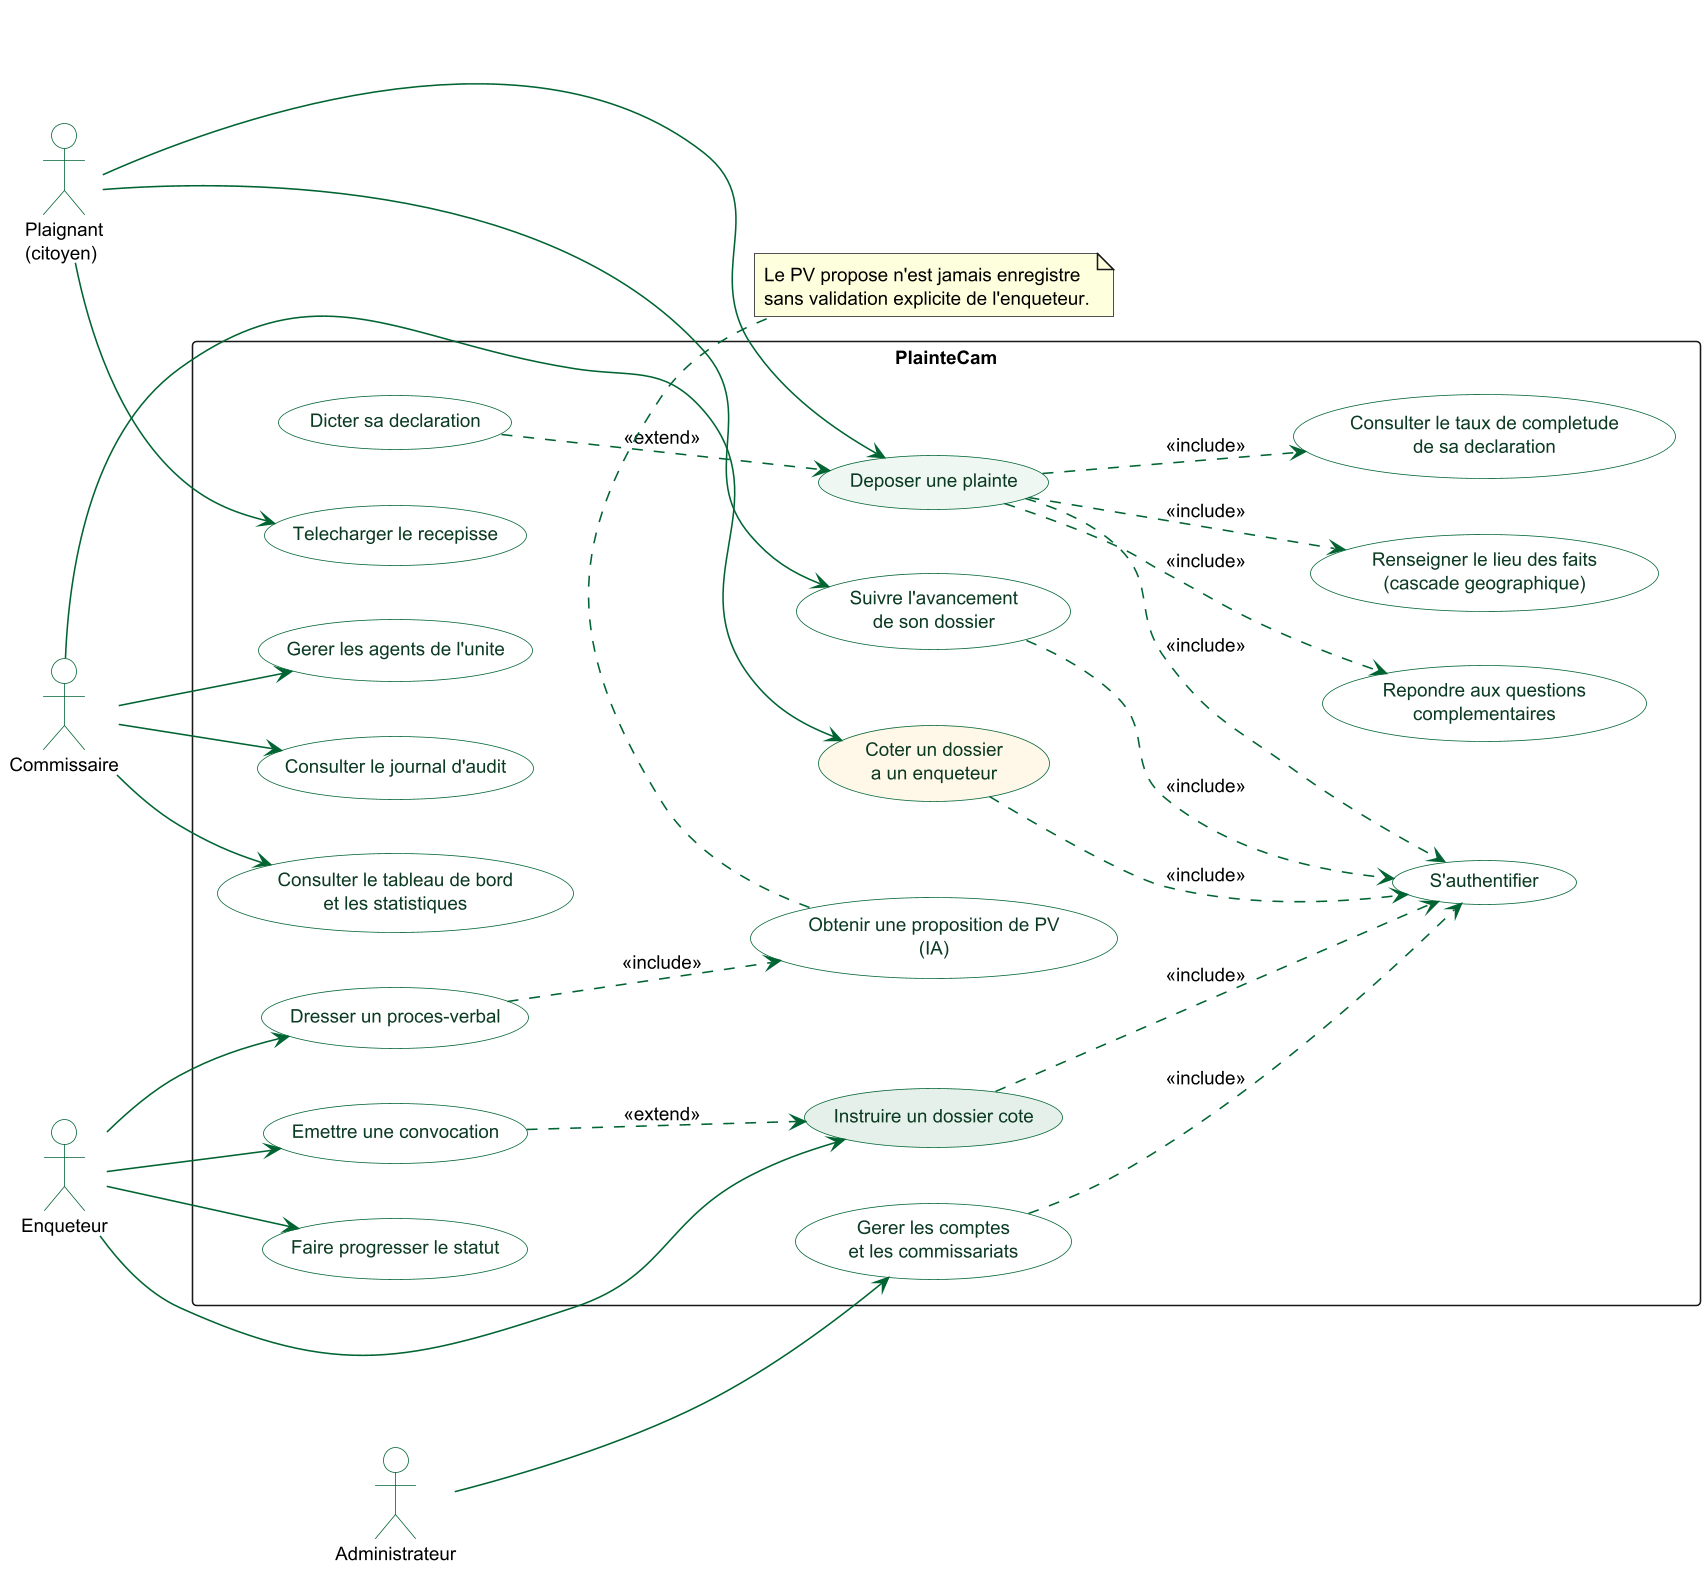
\includegraphics[width=\linewidth]{diagrammes/usecase.png}
    \caption{Diagramme de cas d'utilisation de PlainteCam}
    \label{fig:usecase}
\end{figure}

Deux relations méritent l'attention, car elles portent des règles métier et non de simples commodités d'écriture. La cascade géographique, le calcul du taux de complétude et les questions complémentaires sont des cas \textbf{inclus} dans « déposer une plainte » : ils ne s'exécutent jamais séparément, et le dépôt ne peut aboutir sans eux. De la même façon, « obtenir une proposition de procès-verbal » est inclus dans « dresser un procès-verbal », et non offert comme cas autonome. Le modèle traduit ainsi le principe selon lequel l'intelligence artificielle n'intervient qu'à l'intérieur d'un acte dont l'enquêteur reste responsable. Seule la dictée vocale constitue une \textbf{extension} : elle enrichit le dépôt sans lui être nécessaire.

\section{Démarche adoptée}

Les besoins étant posés, reste à décrire la manière dont le projet a été conduit pour y répondre.

\subsection{Méthodologie de gestion de projet : Agile / Scrum}

Face à la complexité et à l'évolutivité du projet, la méthodologie \textbf{Agile Scrum}~\cite{agile-manifesto} a été adoptée. Cette approche itérative et incrémentale permet de livrer des fonctionnalités en continu, de s'adapter aux retours des parties prenantes et de maîtriser les risques tout au long du développement. Six sprints de trois à quatre semaines ont structuré les six mois de mission.

Le premier sprint a posé les fondations : authentification par jeton, gestion des profils et navigation par rôle. Le deuxième a livré le dépôt de plainte, avec son formulaire en cinq étapes, sa cascade géographique et ses pièces jointes. Le troisième a introduit l'assistance à la déclaration, c'est-à-dire les questions complémentaires, la dictée vocale et la rédaction assistée du procès-verbal. Le quatrième a ouvert l'espace enquêteur, avec les procès-verbaux d'audition et les convocations. Le cinquième a construit l'espace commissaire, sa cotation, ses statistiques et le suivi offert au plaignant. Le sixième et dernier sprint a été consacré à la consolidation : journal d'audit, production des pièces PDF, recette et corrections.

\section{Architecture de la solution}

L'architecture de PlainteCam est présentée sous deux angles complémentaires : ce que la plateforme fait, puis comment elle se découpe en modules. La traduction de ces modules en technologies est traitée au chapitre suivant, car elle relève de la réalisation et non de la conception.

\subsection{Architecture fonctionnelle}

La figure~\ref{fig:archi_fonctionnelle} donne la vue d'ensemble des fonctions de la plateforme. Le cycle de vie d'une plainte s'y lit de gauche à droite en cinq temps, chacun rattaché à l'acteur qui en a la charge : le plaignant \textbf{dépose} sa déclaration, la plateforme \textbf{oriente} le dossier vers le commissariat territorialement compétent, le commissaire le \textbf{cote} à un enquêteur, celui-ci \textbf{instruit} l'affaire puis la \textbf{clôture}.

\begin{figure}[H]
    \centering
    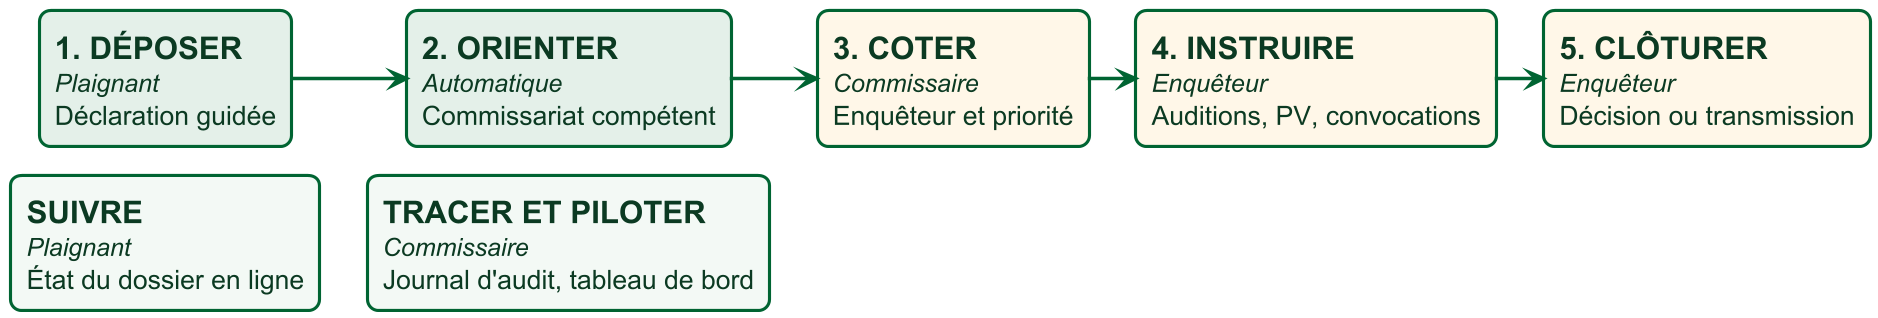
\includegraphics[width=\linewidth]{diagrammes/architecture_fonctionnelle.png}
    \caption{Architecture fonctionnelle : les grandes fonctions de PlainteCam}
    \label{fig:archi_fonctionnelle}
\end{figure}

Deux fonctions échappent à cette séquence parce qu'elles la traversent de bout en bout. Le \textbf{suivi} rend chaque transition visible du plaignant, sans qu'il ait à se déplacer. La \textbf{traçabilité} inscrit ces mêmes transitions au journal d'audit et alimente le tableau de bord du commissaire. Elles ne constituent pas une étape du cycle mais une propriété de l'ensemble, et c'est à ce titre qu'elles figurent à part sur le schéma.

\subsection{Architecture de conception}

La figure~\ref{fig:archi_conception} décompose la solution en modules, indépendamment de toute technologie. Trois ensembles se dégagent autour d'un noyau.

\begin{figure}[H]
    \centering
    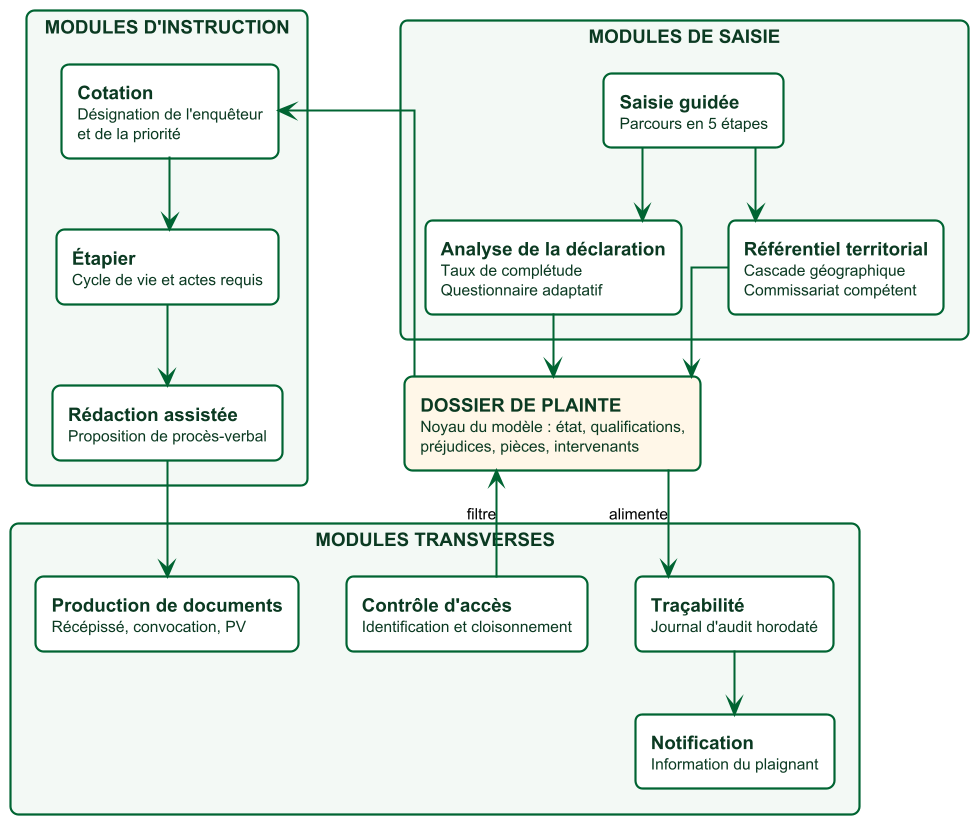
\includegraphics[width=0.86\linewidth]{diagrammes/architecture_conception.png}
    \caption{Architecture de conception : modules et connexions}
    \label{fig:archi_conception}
\end{figure}

Les \textbf{modules de saisie} recueillent la déclaration : le parcours guidé, l'analyse qui en déduit le taux de complétude et les questions à poser, et le référentiel territorial qui détermine l'unité compétente. Les \textbf{modules d'instruction} prennent le relais après le dépôt, avec la cotation, l'étapier qui contraint le cycle de vie, et la rédaction assistée du procès-verbal. Les \textbf{modules transverses} servent les deux précédents : contrôle d'accès, production des documents, traçabilité et notification.

Au centre, le \textbf{dossier de plainte} concentre l'état, les qualifications, les préjudices, les pièces et les intervenants. Tous les modules s'y rattachent, aucun ne dialogue directement avec un autre groupe. Ce choix évite qu'une évolution du parcours de saisie n'affecte l'instruction, et réciproquement.

\section{Modélisation UML}

Les deux diagrammes qui suivent précisent la conception en descendant d'un niveau : le premier décrit les entités manipulées, le second l'enchaînement des échanges entre acteurs et composants.

\subsection{Diagramme de classes}

Le diagramme de classes constitue l'élément central de la modélisation orientée objet. Il décrit comment les entités du domaine interagissent pour concrétiser les différents cas d'utilisation.

\begin{figure}[H]
    \centering
    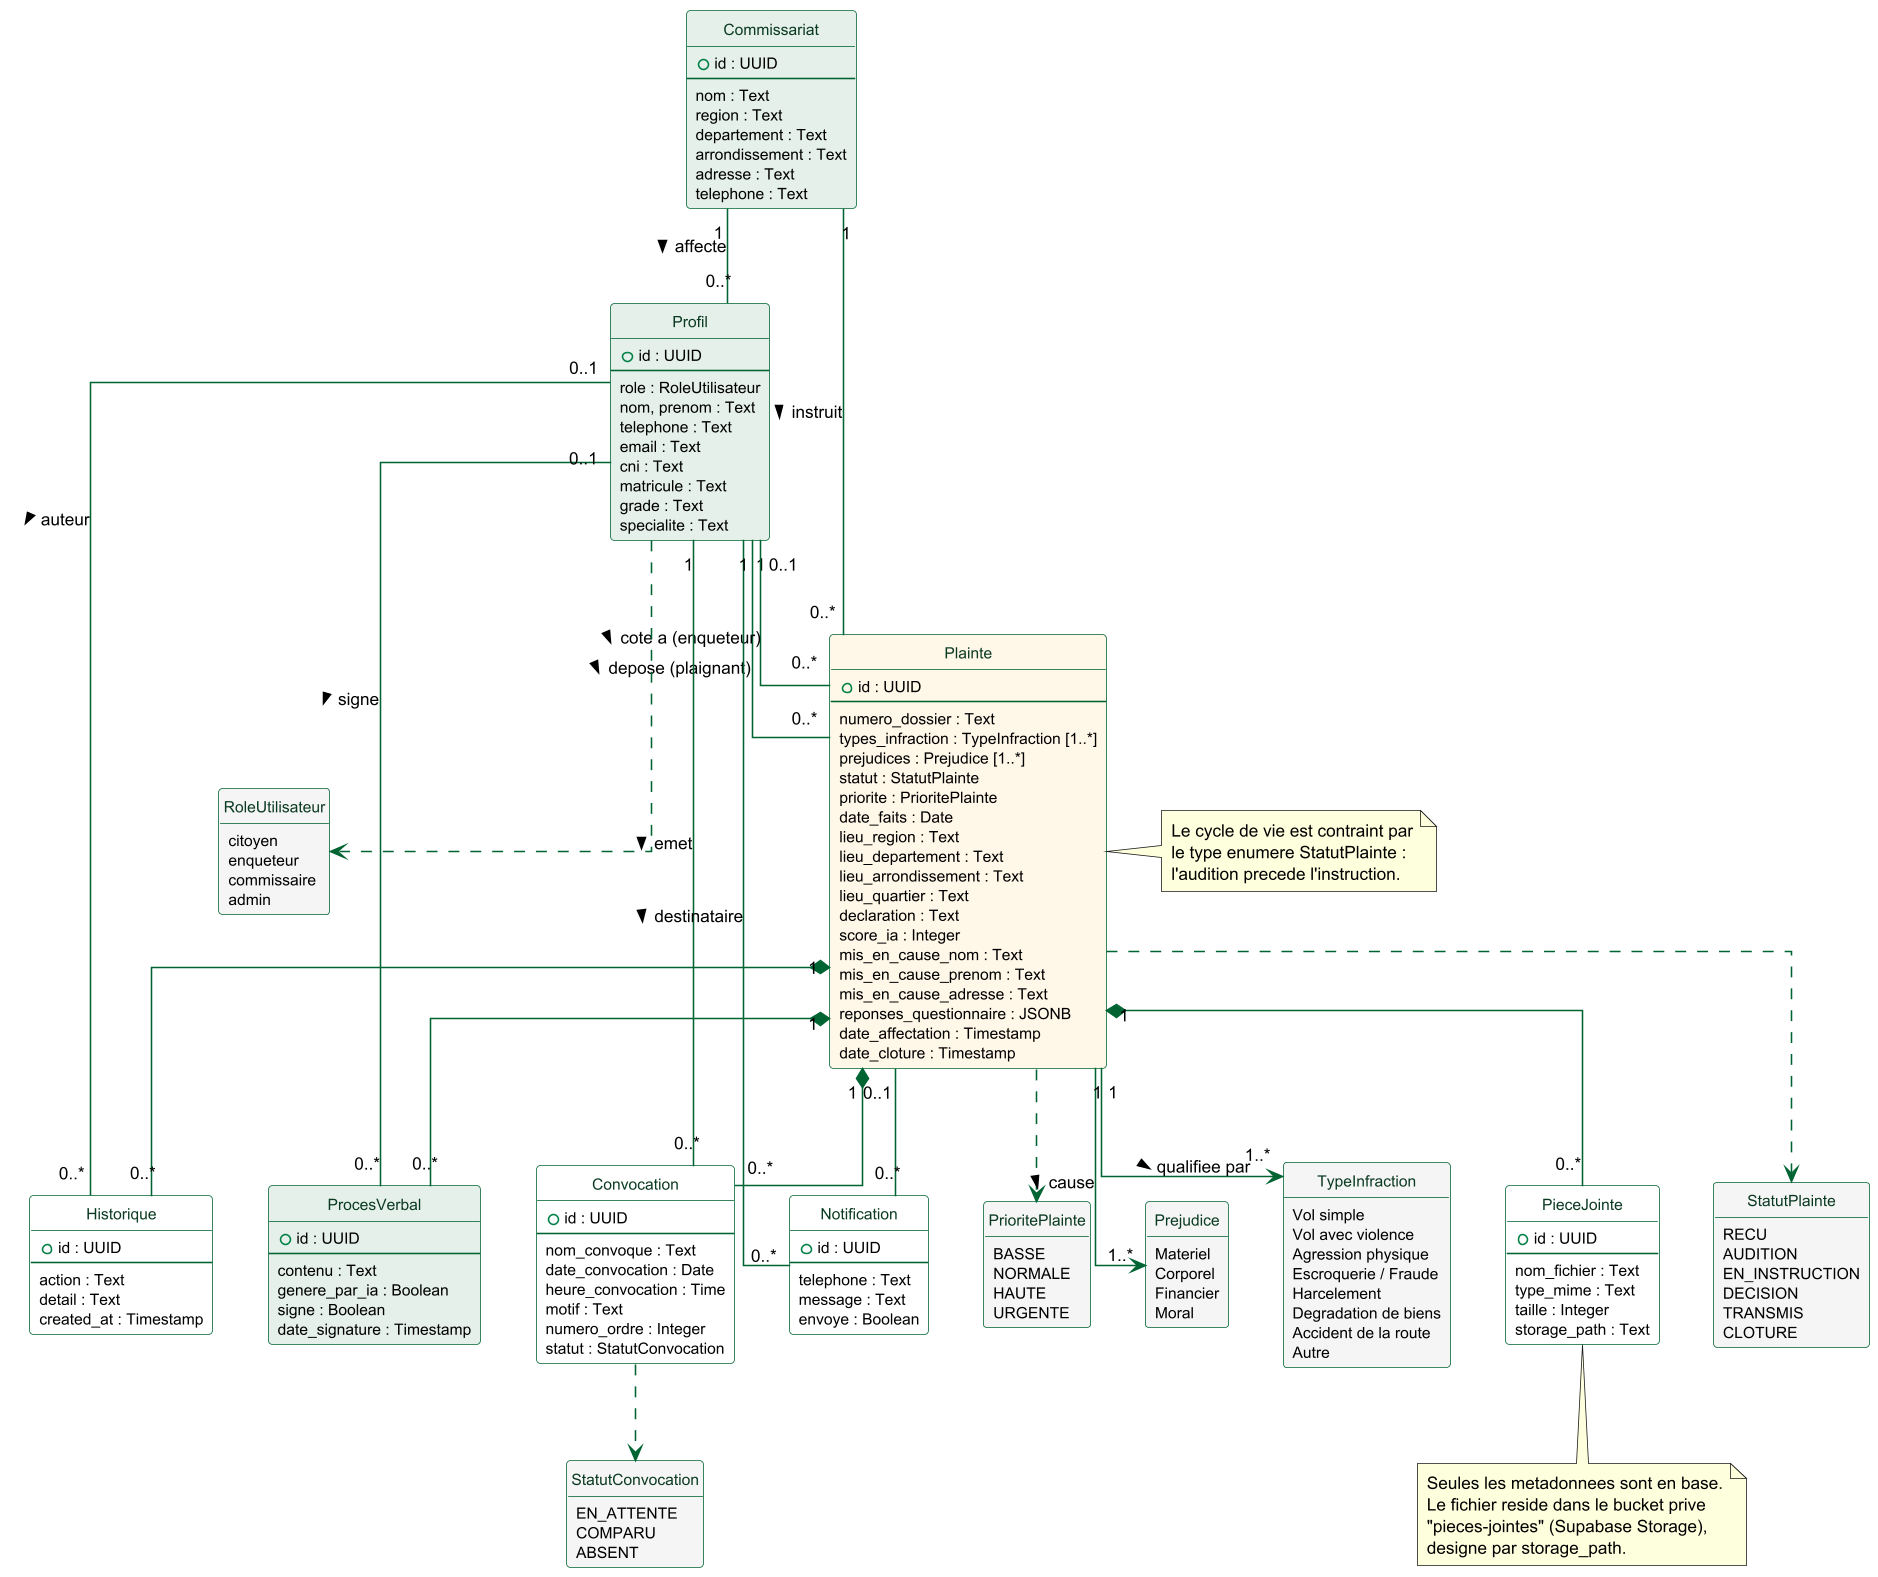
\includegraphics[width=\linewidth]{diagrammes/classe.png}
    \caption{Diagramme de classes : modèle conceptuel de PlainteCam}
    \label{fig:classe}
\end{figure}

\subsection{Diagramme de séquence}

La figure~\ref{fig:sequence} illustre la séquence du dépôt d'une plainte, depuis la saisie guidée jusqu'à la rédaction assistée du procès-verbal.

\begin{figure}[H]
    \centering
    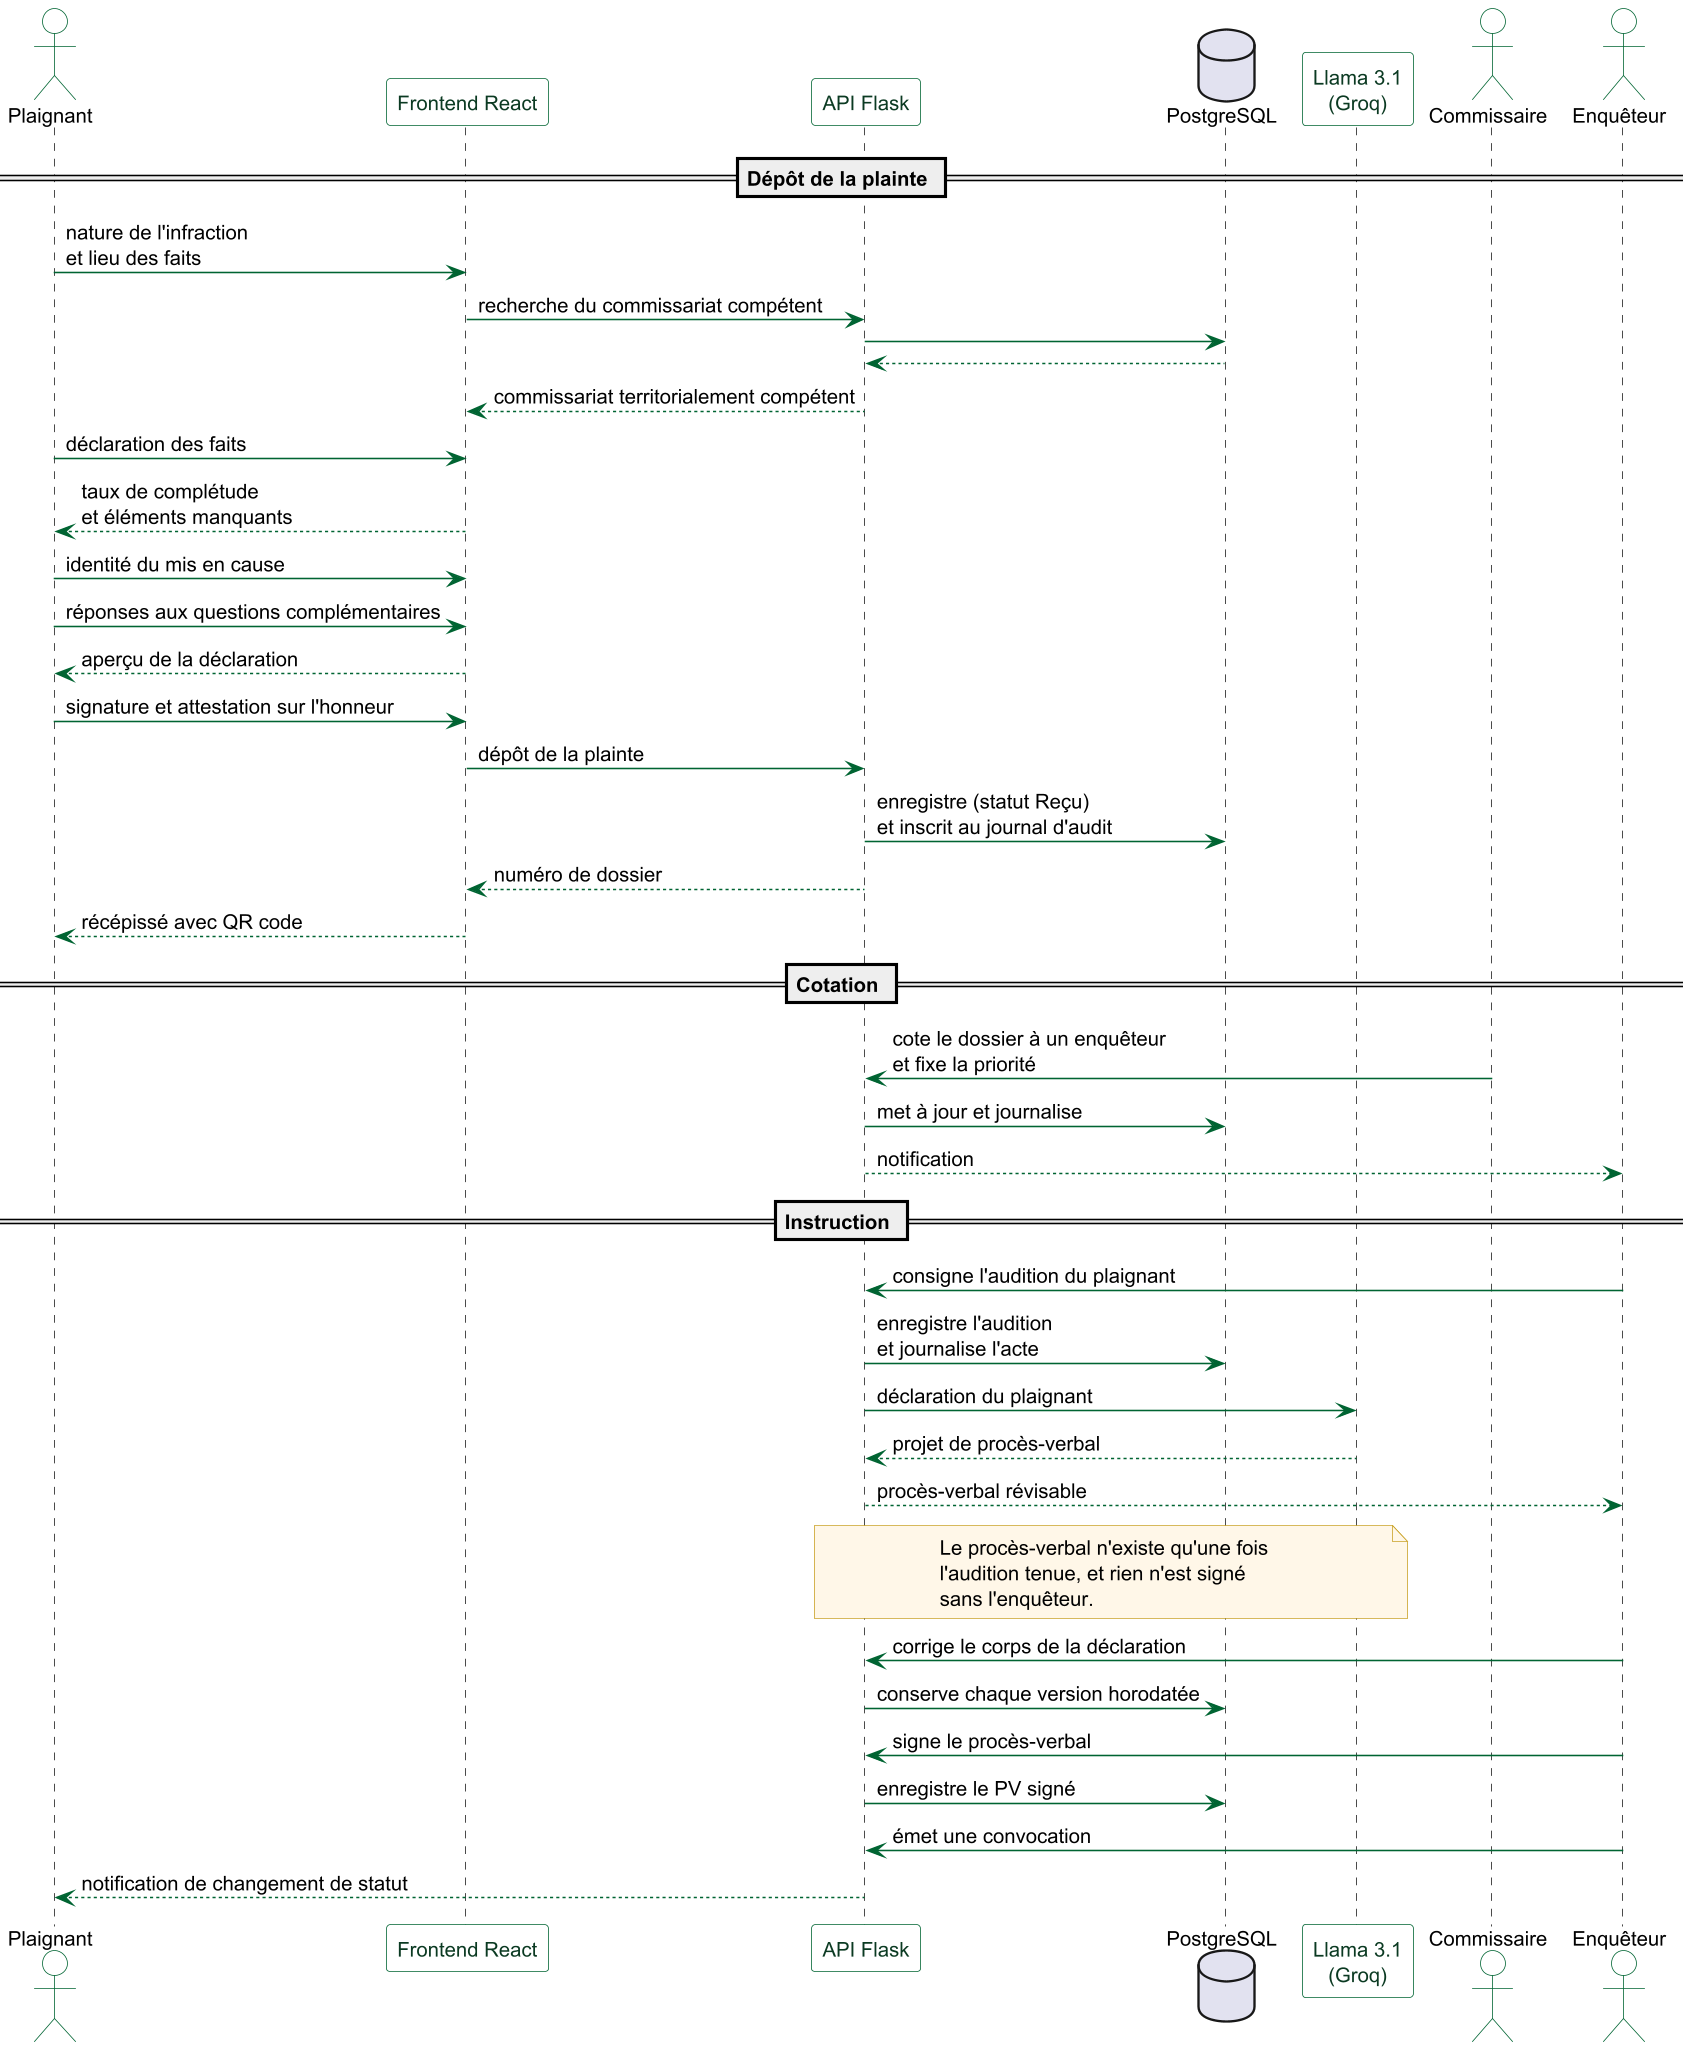
\includegraphics[width=\linewidth]{diagrammes/sequence.png}
    \caption{Diagramme de séquence : dépôt et instruction d'une plainte}
    \label{fig:sequence}
\end{figure}

La conception étant arrêtée, le chapitre suivant en présente la réalisation effective.
